% 请确保文件编码为utf-8,使用XeLaTex进行编译,或者通过overleaf进行编译

\documentclass[answers]{exam}  % 使用此行带有作答模块
% \documentclass{exam} % 使用此行只显示题目

\usepackage{xeCJK}
\usepackage{zhnumber}
\usepackage{graphicx}
\usepackage{hyperref}
\usepackage{amsmath}
\usepackage{amssymb}
\usepackage{mathtools}
\usepackage{booktabs}
\usepackage{enumerate}
\usepackage{enumitem} % 控制列表样式
\usepackage{listings} 

\title{2025模式识别 \\ 作业四}
\date{2025.4.15}
\pagestyle{headandfoot}
\author{人工智能学院 221300079 王俊童}
\firstpageheadrule
\firstpageheader{南京大学}{2025模式识别}{作业四}
\runningheader{南京大学}
{2025模式识别}
{作业四}
\runningheadrule
\firstpagefooter{}{第\thepage\ 页(共\numpages 页)}{}
\runningfooter{}{第\thepage\ 页(共\numpages 页)}{}

% no box for solutions
% \unframedsolutions
\def \x \mathbf{x}


\setlength\linefillheight{.5in}

% \renewcommand{\solutiontitle}{\noindent\textbf{答:}}
\renewcommand{\solutiontitle}{\noindent\textbf{解:}\par\noindent}

\renewcommand{\thequestion}{\zhnum{question}}
\renewcommand{\questionlabel}{\thequestion .}
\renewcommand{\thepartno}{\arabic{partno}}
\renewcommand{\partlabel}{\thepartno .}

\def\dist{{\mathrm{dist}}}
\def\x{{\boldsymbol{x}}}
\def\w{{\boldsymbol{w}}}


\begin{document}
% \normalsize
\maketitle
221300079 王俊童,人工智能学院
\section{问题一}
\begin{enumerate}[label=\alph*.] 
    \item 我们假设对于i样本,K近邻$z_{i1},\cdots, z_{iK}$,设$Z_i = [z_{i1}-z_i,\cdots,z_{iK} - z_i]$,有重构误差:
    \begin{equation*}
        \|\sum_{j=1}^{K} w_{ij}(z_{ij} - z_i)\|^2 = w_i^T C_i w_i = w_i^T Z_i^T Z_i w_i
    \end{equation*}
    所以优化问题如下:
    \begin{align*}
        \min_{w_i} &\qquad w_i^T C_i w_i\\
                   &\qquad s.t. \sum_{j=1}^{K} w_{ij} = 1\\ 
    \end{align*}
    根据拉格朗日乘子法:
    \[
        L(w_i, \lambda) = w_i^T C_i w_i - \lambda(\mathbf{1}^T w_i - 1), \quad  C_i w_i = \frac{\lambda}{2}\mathbf{1},\quad \mathbf{1}^T w_i = 1
    \]
    解得:
    \[
        \lambda = \frac{2}{\mathbf{1}^T C_i^{-1} \mathbf{1}}, \quad w_i = \frac{C_i^{-1} \mathbf{1}}{\mathbf{1}^T C_i^{-1} \mathbf{1}}
    \]
    \item 根据第一问,我们逐个进行证明:
    \begin{itemize}
        \item 旋转不变性,令$z_j' = Qz_j$,因为Q是正交矩阵$Q^TQ = I$:
        \[
            \|Qz_i - \sum_{j}w_{ij}Qz_j\|^2 = \|Q(z_i - \sum_{j}w_{ij}z_j)\|^2 = \|(z_i - \sum_{j}w_{ij}z_j)\|^2 
        \]
        \item 平移不变性,令$z_j'= z_j + t$:
        \[
            \|z_i +t - \sum_{j}w_{ij}(z_j + t)\|^2 = \|z_i - \sum_{j}w_{ij}z_j + t - (\sum_{j} w_ij)t\| =  \|(z_i - \sum_{j}w_{ij}z_j)\|^2 
        \]
        \item 缩放不变性,令$z_j' = sz_j$:
        \[
            \|sz_i - \sum_{j}w_{ij}sz_j\|^2 = \|s^2(z_i - \sum_{j}w_{ij}z_j)\|^2 \rightarrow  \|(z_i - \sum_{j}w_{ij}z_j)\|^2 
        \]
        其中缩放倍数s并不改变优化目标。
    \end{itemize}
    \item 首先这么修改之后,因为这个问题本质是一个manifold learning 的问题。优化目标不改变,仍然是在一个低维空间里面重构一个权重,保留了局部的manifold的结构。
    
    对于两个约束条件,第一个等于0的约束相当于约束了所有低维向量的均值为0,消除了平移自由度,这样低维表示都在原点附近了。

    对于第二个条件,相当于正交而且归一化,这样协方差就是单位了,消除了缩放,而且整个低维都在一个单位球上,所以表示也被规范化了。所以好像旋转自由度也被消除了。

    其实我个人还有一个理解是,这个问题对于旋转自由度其实不是特别的敏感,因为好像旋转自由度对于这个问题影响真的不大,似乎最优解都是在一个点附近了。

    \item 不妨由厦门政府,我们从9.52开始算:
    \[
        L(y) = \sum_{i=1}^{n}\|y_i - \sum_{j} w_{ij}y_j\|^2 = \|Y - WY\|^2
    \]
    这个问题是等价的事,我们可以令$\hat{y} = \sum_{j} w_{ij}y_j$,然后写成矩阵形式. 可以化简 
    \[
        L(y) = Tr(Y^T(I - W)^T(I- W)Y) = Tr(Y^T M Y) = \sum_{i,j} M_{ij} y_i^T y_j
    \]
    \item 首先证明M是一个半正定的,假设有v:
    \[
        v^T M v= \|(I - W)v\|^2 \geq 0
    \]
    然后为什么1向量是一个特征向量呢:
    \[
        (I - W)\mathbf{1} = 1 - W1 = \mathbf{0}, \quad \sum_{j}w_{ij} = 1
    \]
    所以证明完了,然后这个第一个按照升序排序的就是0对应的特征向量。因为我们在降维的时候实际上对于的是d个最小的非零特征值的特征向量。所以这个对于平移自由度的约束其实是没用的,所以要舍弃,无意义。
    \item 尝试看看但是:
    \begin{figure*}[h!]
        \centering
        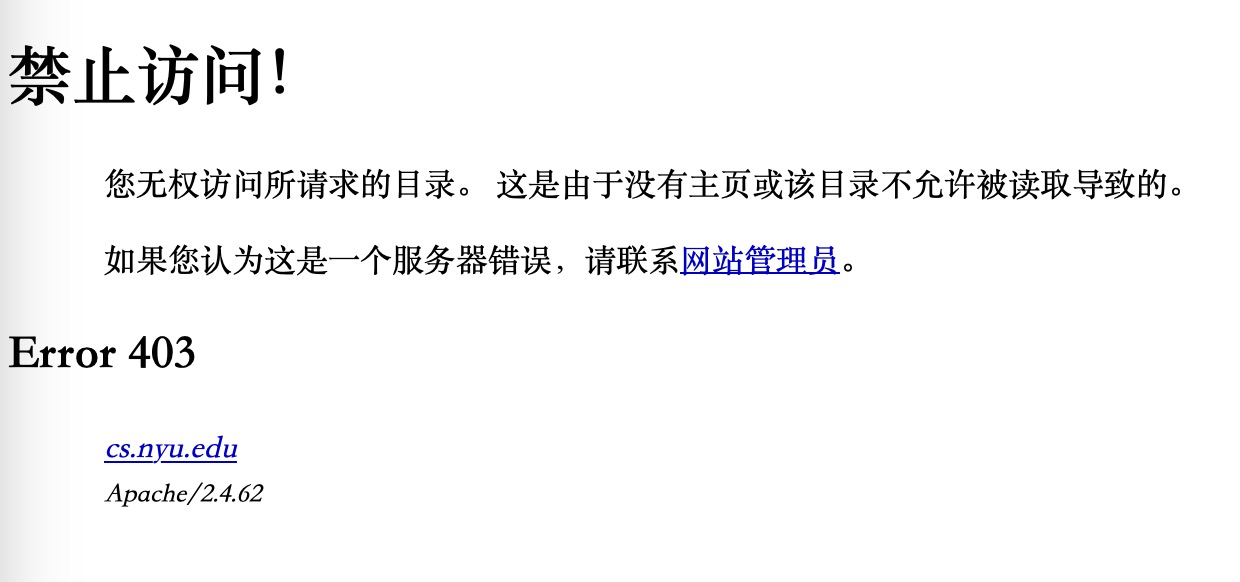
\includegraphics[scale=0.3]{forbid.png}
        \caption{forbidden}
        \label{forbidden}
    \end{figure*}
\end{enumerate}

\section{问题二}
\begin{enumerate}[label=\alph*.] 
    \item \[
        1 - \sigma(x) = 1 - \frac{1}{1 + e^{-x}} = \frac{e^{-x}}{1 + e^{-x}} = \frac{1}{1 + e^{x}} = \sigma(-x)
    \]  
    \item \[
        \sigma(x)' = \frac{e^{-x}}{(1 + e^{-x})^2} = \sigma(x)(1 - \sigma(x))
    \]
    \begin{figure*}[h!]
        \centering
        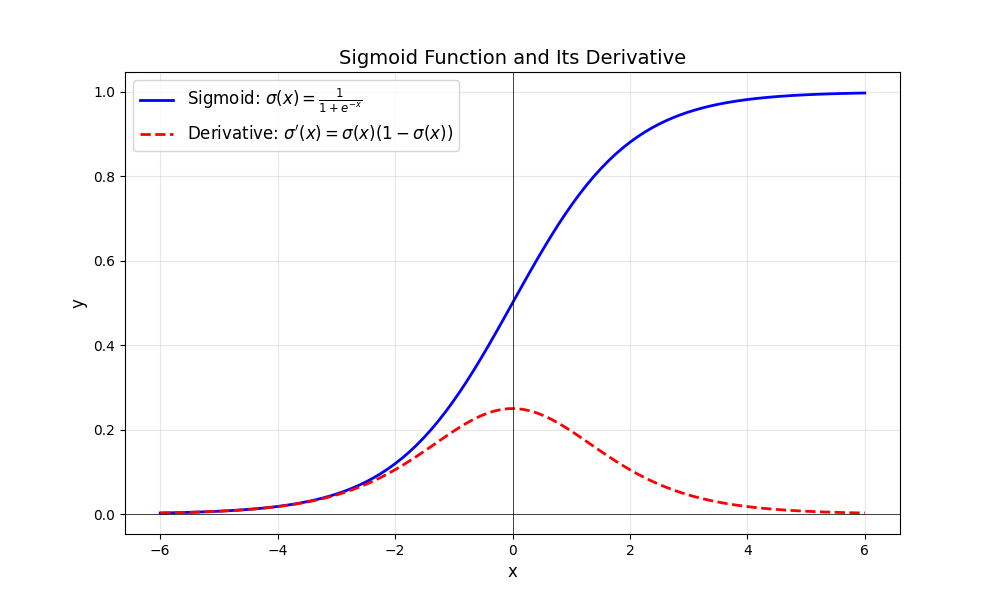
\includegraphics[scale=0.5]{sigmoid.png}
        \caption{sigmoid}
        \label{sigmoid}
    \end{figure*}
    \item 因为神经网络是一个多层的,并且是一层一层求导往后算的,所以我们目前看第i层的网络节后
    \[
        y_j^{(i)} = \sigma'(z_j^{(i)})
    \]
    所以根据上面的图可以看到,这个导数是一个只有最大值0.25的情况,并且越往旁边数据就越接近0,有大一点的值的位置是非常少的。所以我们如果从头开始算L次,梯度会变得非常非常少,这就会导致深度神经网络中的梯度消失问题。结果越趋近于0,问题越大。
\end{enumerate}

\section{问题三}
\begin{enumerate}[label=\alph*.] 
    \item 1, 1, 2, 3, 5, 8
    \item 可以求解$F_n - F_{n-1} - F_{n-2} = 0$, 我们假设通解如下:
    \[
        F_n= A\alpha^n + B\beta^n
    \]
    所以根据特征方程可以得到:
    \[
        r^2 - r - 1 =0, \quad \alpha = \frac{1+\sqrt{5}}{2} ,\beta = \frac{1 - \sqrt{5}}{2}
    \]
    因为根据前两个斐波那契数可以得到:
    \begin{equation*}
        \begin{cases*}
            A \alpha + B\beta = 1\\
            A \alpha^2 + B\beta^2 = 1
        \end{cases*}
    \end{equation*}
    可以解答得到:$A = \frac{1}{\alpha - \beta}, B = \frac{-1}{\alpha - \beta}$,所以得到:
    \[
        F_n = \frac{\alpha^n - \beta^n}{\alpha - \beta}
    \]
    \item 我们首先证明这个式子,用数学归纳法;
    \begin{itemize}
        \item 首先为1的情况:$F_3 = 2$, $F_1 = 1$,所以满足。
        \item 假设n也满足
        \item 看n+1的情况:
        \[
            \sum_{i=1}^{n+1} F_i = (\sum_{i=1}^{n} F_i) + F_{n+1} = F_{n+2} - 1 + F_{n+1} = F_{n+3} - 1
        \]
    \end{itemize}
    然后我们看
    \[
        p_i = \frac{F_i}{F_{n+2} - 1}, i=1,2,\cdots, n
    \]
    首先这个东西肯定非负,然后在0-1之间,然后还满足:
    \[
        \sum p_i = \frac{\sum F_i}{F_{n+2} -1} = 1
    \]
    \item 用数学归纳法证明:
    \begin{itemize}
        \item n=1, $\sum 1F_1 = F_3 - F_4 + 2 = 1$
        \item n=k,假设也满足这个式子
        \item n=k+1:要证明  
        \[
            \sum_{i=1}^{k+1} iF_i = (k+1)F_{k+3} - F_{k+4} + 2
        \]
        \[
            \sum_{i=1}^{k+1} iF_i = \sum_{i=1}^{k} iF_i + (k+1)F_{k+1} = kF_{k+2} - F_{k+3} + 2 + (k+1)F_{k+1}
        \]
        \[
            = (k+1)(F_{k+1}+F_{k+2}) - (F_{k+2} +F_{k+3}) + 2 = (k+1)F_{k+3} - F_{k+4} + 2
        \]
        所以证明完毕
    \end{itemize}
    \item 首先这个p为$F_1,\cdots,F_5$ = $\{\frac{1}{12}, \frac{1}{12}, \frac{2}{12},\frac{3}{12}, \frac{5}{12}\}$
    所以霍夫曼树如下:
    \begin{lstlisting}[language=python]
          [12]
        /      \
      [5]       [7]
      (E)     /     \
          [3]       [4]
          (D)     /     \
               [2]     [2]
               (C)   /     \
                    (A)    (B)
    \end{lstlisting}
    其中:$E: 0, D: 10, C: 110, A: 1110, B: 1111$.
    \item 根据观察,我们可以看到由于斐波那契数列的单调性质,从n=2开始,就满足每一个都比上一个大,所以树一定是不平衡的,意思是,我们的$F_1,...,F_n$ 对应的编码长度是:$n-1,n-1,n-2,...,1$,所以满足:
    \[
        B = p*l = \frac{1}{F_{n+2} -1}*E, \quad E = (\sum_{i=2}^{n} F_i(n-i+1) + (n-1))
    \]
    因为:
    \[
        \sum_{i=2}^{n} F_i n = F_{n+2} - 2, \quad \sum_{i=2}^{n} iF_i = nF_{n+2} - F_{n+3} + 1
    \]
    所以可以化简为:
    \[
        E = n(F_{n+2} - 2) - (nF_{n+2} -F_{n+3} + 1) + (F_{n+2} - 2) + n-1 = F_{n+3} + F_{n+2} -n -4 = F_{n+4} - (n+4)
    \]
    \[
        B = \frac{F_{n+4} - (n+4)}{F_{n+2} -1}
    \]
    \item 因为$F_n = \frac{\alpha^n - \beta^n}{\sqrt{5}}$因为有一个$\frac{1-\sqrt{5}}{2} < 0$,所以$n\rightarrow \infty, \quad F_n \sim \frac{\alpha^n}{\sqrt{5}}$
    
    所以:
    \[
        B_n \approx \frac{\frac{\alpha^{n+4}}{\sqrt{5}} - (n+4)}{ \frac{\alpha^{n+2}}{\sqrt{5}} - 1}
    \]
    可以忽略低阶项:
    \[
        B_n \approx \frac{\frac{\alpha^{n+4}}{\sqrt{5}} }{ \frac{\alpha^{n+2}}{\sqrt{5}}} = (\frac{1 + \sqrt{5}}{2})^2 \approx 2.618
    \]
    所以平均需要2.618的比特来编码。
\end{enumerate}

\section{问题四}
\begin{enumerate}[label=\alph*.] 
    \item 根据积分图的定义可以得到B:
    \[  
        \begin{pmatrix}
            1 & 1 & -1 \\
            2 & 3 & 1  \\
            3 & 4 & 6  \\
        \end{pmatrix}
        \rightarrow    
        \begin{pmatrix}
            1 & 2 & 1 \\ 
            3 & 7 & 7 \\
            6 & 14 & 20 \\
        \end{pmatrix}
    \]
    \item 我们根据积分图的定义,确实可以有一种动态规划的算法:
    \[
        B(i,j) = A(i, j) + B(i-1, j) + B(i,j -1) - B(i-1, j-1)
    \]
    根据动态规划算法来看,整个算法确实是$O(m*n)$的,因为每一个位置的计算都是$O(1)$的,然后确实是线性的。其实是两个大矩形相加减去重复部分就行。
    \item 那么根据之前我们的积分图来说,任意的矩阵$i_1i_2j_1j_2$都可以$O(1)$算出来,我们只需要做3次加减法即可,相当于:
    \[
        S  =B(i_2,j_2) - B(i_1- 1, j_2) - B(i_2, j_1-1) + B(i_1-1, j_1-1)
    \]  
    所以是$O(1)$的。
\end{enumerate}


\section{问题五}
\begin{enumerate}[label=\alph*.] 
    \item 我们只需要证明一个问题即可证明独立性:$p(A, B|C) = p(A|C)p(B|C)$:
    \[
        p(A, B|C) = \frac{p(A, B, C)}{p(C)} = \frac{p(C|A)p(B|C)p(C)}{p(C)} = \frac{p(A, C)}{p(C)} p(B|C)=p(A|C)p(B|C)
    \]
    \item 1.2同理:
    \[
        p(A, B|C) = \frac{p(A, B, C)}{p(C)} = \frac{p(B)p(C|B)p(A|C)}{p(C)} = \frac{p(B, C)}{p(C)} p(A|C)=p(A|C)p(B|C)
    \]
    \item 1.3同理:
    \[
        p(A, B|C) = \frac{p(A, B, C)}{p(C)} = \frac{p(C)p(A|C)p(B|C)}{p(C)} = p(A|C)p(B|C)
    \]
    \item 
\end{enumerate}

\end{document}